\documentclass[tikz]{standalone}

\usepackage{tgheros}
\renewcommand{\labelitemi}{{\rmfamily \textbullet}} % Prevents problem with bullet in tgheros
\renewcommand{\familydefault}{\sfdefault} % Makes the default text sans serif

\definecolor{aublue}{RGB}{25,33,129}
\definecolor{aured}{RGB}{244,28,31}

\begin{document}
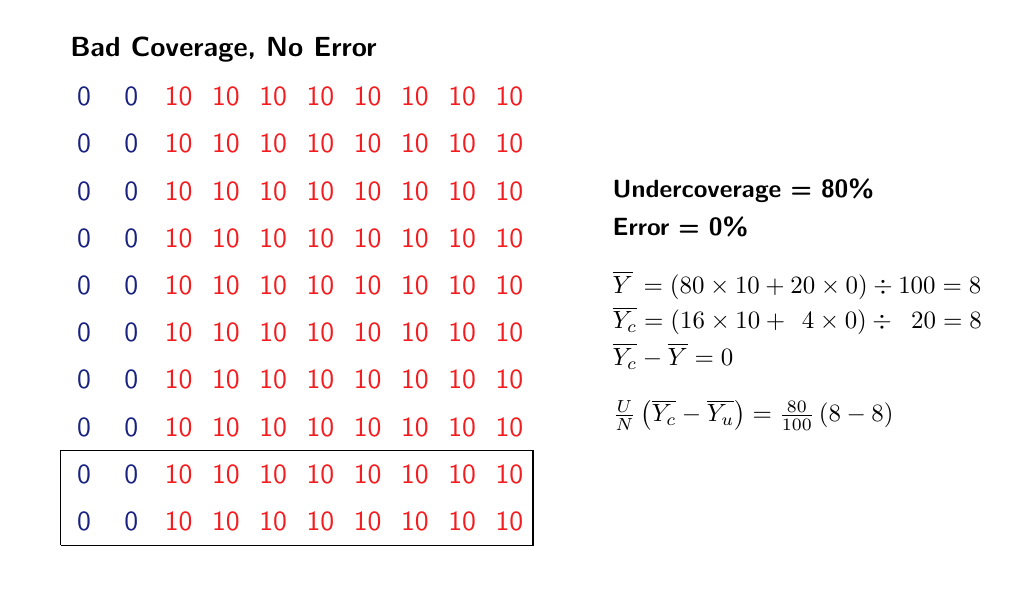
\begin{tikzpicture}[scale=.6]
\node at (.5,11) [anchor=west] {\textbf{Bad Coverage, No Error}};
	\foreach \y in {1,2,3,4,5,6,7,8,9,10} {
		\foreach \x in {1,2} {
		\node at (\x,\y) [color=aublue,align=center] {0};	
			}
		\foreach \x in {3,4,5,6,7,8,9,10} {
		\node at (\x,\y) [color=aured,align=center] {10};	
			}
		}

\draw (0.5,.5) -- (10.5,.5) -- (10.5,2.5) -- (0.5,2.5) -- (0.5,.5);
\node at (12,8) [right,scale=.9] {\textbf{Undercoverage = 80\%}};
\node at (12,7.25) [right,scale=.9] {\textbf{Error = 0\%}};
\node at (12,6) [right,scale=.9] {$\overline{Y} \, = \left(80\times 10 + 20\times 0\right) \div 100 =  8$};
\node at (12,5.25) [right,scale=.9] {$\overline{Y_c} = \left(16\times 10 + \;\, 4\times 0\right) \div \;\;20 = 8$};
\node at (12,4.5) [right,scale=.9] {$\overline{Y_c} - \overline{Y} = 0$};
\node at (12,3.25) [right,scale=.9]{$ \frac{U}{N}\left(\overline{Y_c} - \overline{Y_u}\right) = \frac{80}{100}\left(8 - 8\right)$};\node at (0,0) {};
\end{tikzpicture}
\end{document}